\begin{figure}[htbp]
    \centering
    \resizebox{0.92\textwidth}{!}{%
    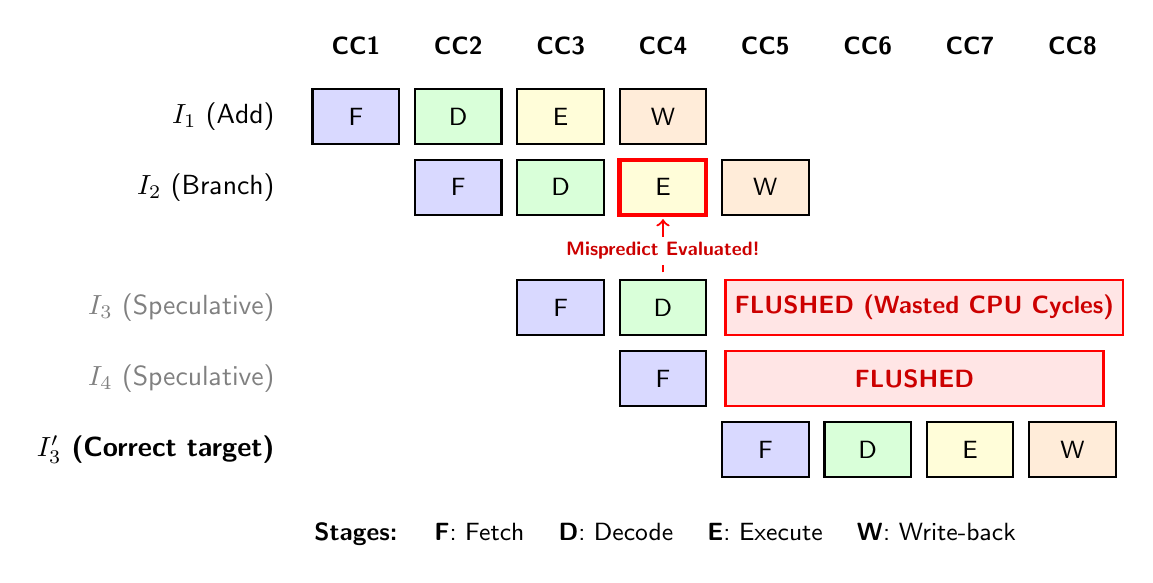
\begin{tikzpicture}[
        x=1.3cm, y=-0.9cm, % scale grid parameters
        font=\sffamily\small,
        stage/.style={rectangle, draw=black, thick, minimum width=1.1cm, minimum height=0.7cm, align=center},
        f/.style={stage, fill=blue!15},
        d/.style={stage, fill=green!15},
        e/.style={stage, fill=yellow!15},
        w/.style={stage, fill=orange!15},
        flush/.style={rectangle, draw=red, thick, fill=red!10, text=red!80!black, minimum width=4.8cm, minimum height=0.7cm, font=\sffamily\bfseries\small},
        label/.style={anchor=east, font=\sffamily}
    ]

    % X-axis headers (Clock cycles)
    \foreach \c in {1,...,8} {
        \node at (\c, 0) {\textbf{CC\c}};
    }

    % Row 1: Normal instruction
    \node[label] at (0.3, 1) {$I_1$ (Add)};
    \node[f] at (1, 1) {F};
    \node[d] at (2, 1) {D};
    \node[e] at (3, 1) {E};
    \node[w] at (4, 1) {W};

    % Row 2: Branch instruction
    \node[label] at (0.3, 2) {$I_2$ (Branch)};
    \node[f] at (2, 2) {F};
    \node[d] at (3, 2) {D};
    \node[e, draw=red, ultra thick] at (4, 2) {E}; % Resolved in CC4
    \node[w] at (5, 2) {W};

    % Annotation for mispredict
    \draw[->, thick, red] (4, 3.2) -- (4, 2.45);
    \node[color=red!80!black, font=\sffamily\bfseries\scriptsize, align=center, fill=white, inner sep=2pt] at (4, 2.9) {Mispredict Evaluated!};

    % Row 3: Speculative instruction 1
    \node[label, color=gray] at (0.3, 3.7) {$I_3$ (Speculative)};
    \node[f] at (3, 3.7) {F};
    \node[d] at (4, 3.7) {D};
    \node[flush, anchor=west] at (4.6, 3.7) {FLUSHED (Wasted CPU Cycles)};

    % Row 4: Speculative instruction 2
    \node[label, color=gray] at (0.3, 4.7) {$I_4$ (Speculative)};
    \node[f] at (4, 4.7) {F};
    \node[flush, anchor=west] at (4.6, 4.7) {FLUSHED};

    % Row 5: Correct recovery instruction
    \node[label, font=\sffamily\bfseries] at (0.3, 5.7) {$I_3'$ (Correct target)};
    \node[f] at (5, 5.7) {F}; % Starts fresh in CC5
    \node[d] at (6, 5.7) {D};
    \node[e] at (7, 5.7) {E};
    \node[w] at (8, 5.7) {W};

    % Legend
    \node[anchor=west, font=\sffamily\small] at (0.5, 6.9) {\textbf{Stages:} \quad \textbf{F}: Fetch \quad \textbf{D}: Decode \quad \textbf{E}: Execute \quad \textbf{W}: Write-back};

    \end{tikzpicture}
    }
    \caption{A chronological textbook view of a pipeline flush across discrete Clock Cycles (CC). When the branch ($I_2$) evaluates its condition at the Execute phase (CC4) and discovers a misprediction, all speculatively fetched incoming instructions ($I_3$, $I_4$) are forcefully discarded. The pipeline violently stalls until the correct target instructions ($I_3'$) are fetched and advance through the queue.}
    \label{fig:pipeline_flush}
\end{figure}
